\subsection{Behavioral Clustering}

\begin{frame}
\frametitle{What Are Regexes Used For?}
\begin{figure}[ht]
  \centering
  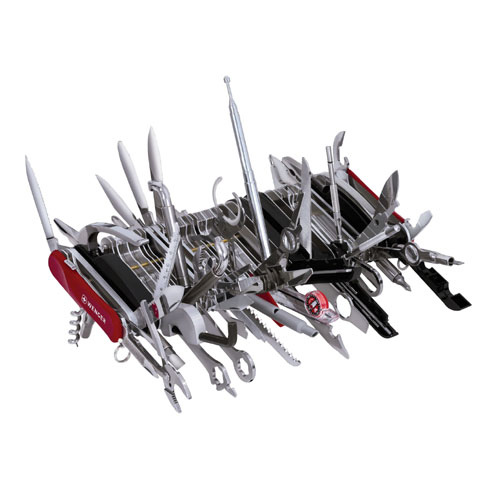
\includegraphics[scale=0.7]{nontex/illustrations/swissArmyMess.jpg}
  \label{fig:whatUsedFor}
\end{figure}
\end{frame}
\note[itemize]{
    \item https://c2.staticflickr.com/4/3057/2383953694_4b148d0a61.jpg
}

%------------------------------------------------



\begin{frame}
\frametitle{How to Categorize Regex Usages}
\begin{enumerate}
\item \sout{thorough inspection of 55K utilizations}
\item \sout{unguided manual categorization of 4,694 regexes (in 2 or more projects), without objective basis}
\item \sout{cluster by syntactic similarity like Jaccard or longest substring}
\item \sout{formal analytical subsumption, using hampi (94\%?) cannot get it to work}
\item \sout{formal analytical subsumption, using brics (30\% or less)}
\item Chosen technique: cluster by behavioral similarity using Rex (61\%)
\end{enumerate}
\end{frame}
\note[itemize]{
    \item has2: 4694
    \item hampi:
    \item bricsOK: 1415? 30\% or less
    \item rexOK-actual: 2871 61\%
}

%------------------------------------------------

\begin{frame}
\frametitle{Measuring Behavioral Similarity}
\begin{figure}[ht]
  \centering
  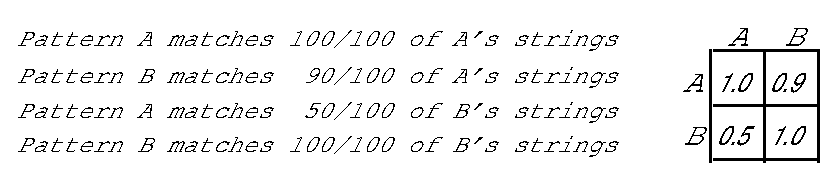
\includegraphics[scale=0.65]{nontex/illustrations/minimalMatrix.eps}
  \label{fig:minimalMatrix}
\end{figure}

\begin{columns}[t] % The "c" option specifies centered vertical alignment while the "t" option is used for top vertical alignment
\column{.5\textwidth} % Left column and width
\begin{figure}[h]
  \centering
  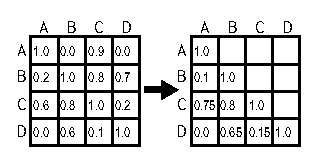
\includegraphics[scale=1]{nontex/illustrations/matrixToGraph.eps}
  \label{fig:matrixToGraph}
\end{figure}
\column{.5\textwidth} % Right column and width
\begin{center}
Rex generates 400 strings\\
for each regex.\\
Convert scores to half-matrix\\
to make abc file for mcl.
\end{center}
\end{columns}
\end{frame}

\note[itemize]{
    \item ok, simple
}

%------------------------------------------------

\begin{frame}
\frametitle{MCL example}
\begin{figure}[ht]
  \centering
  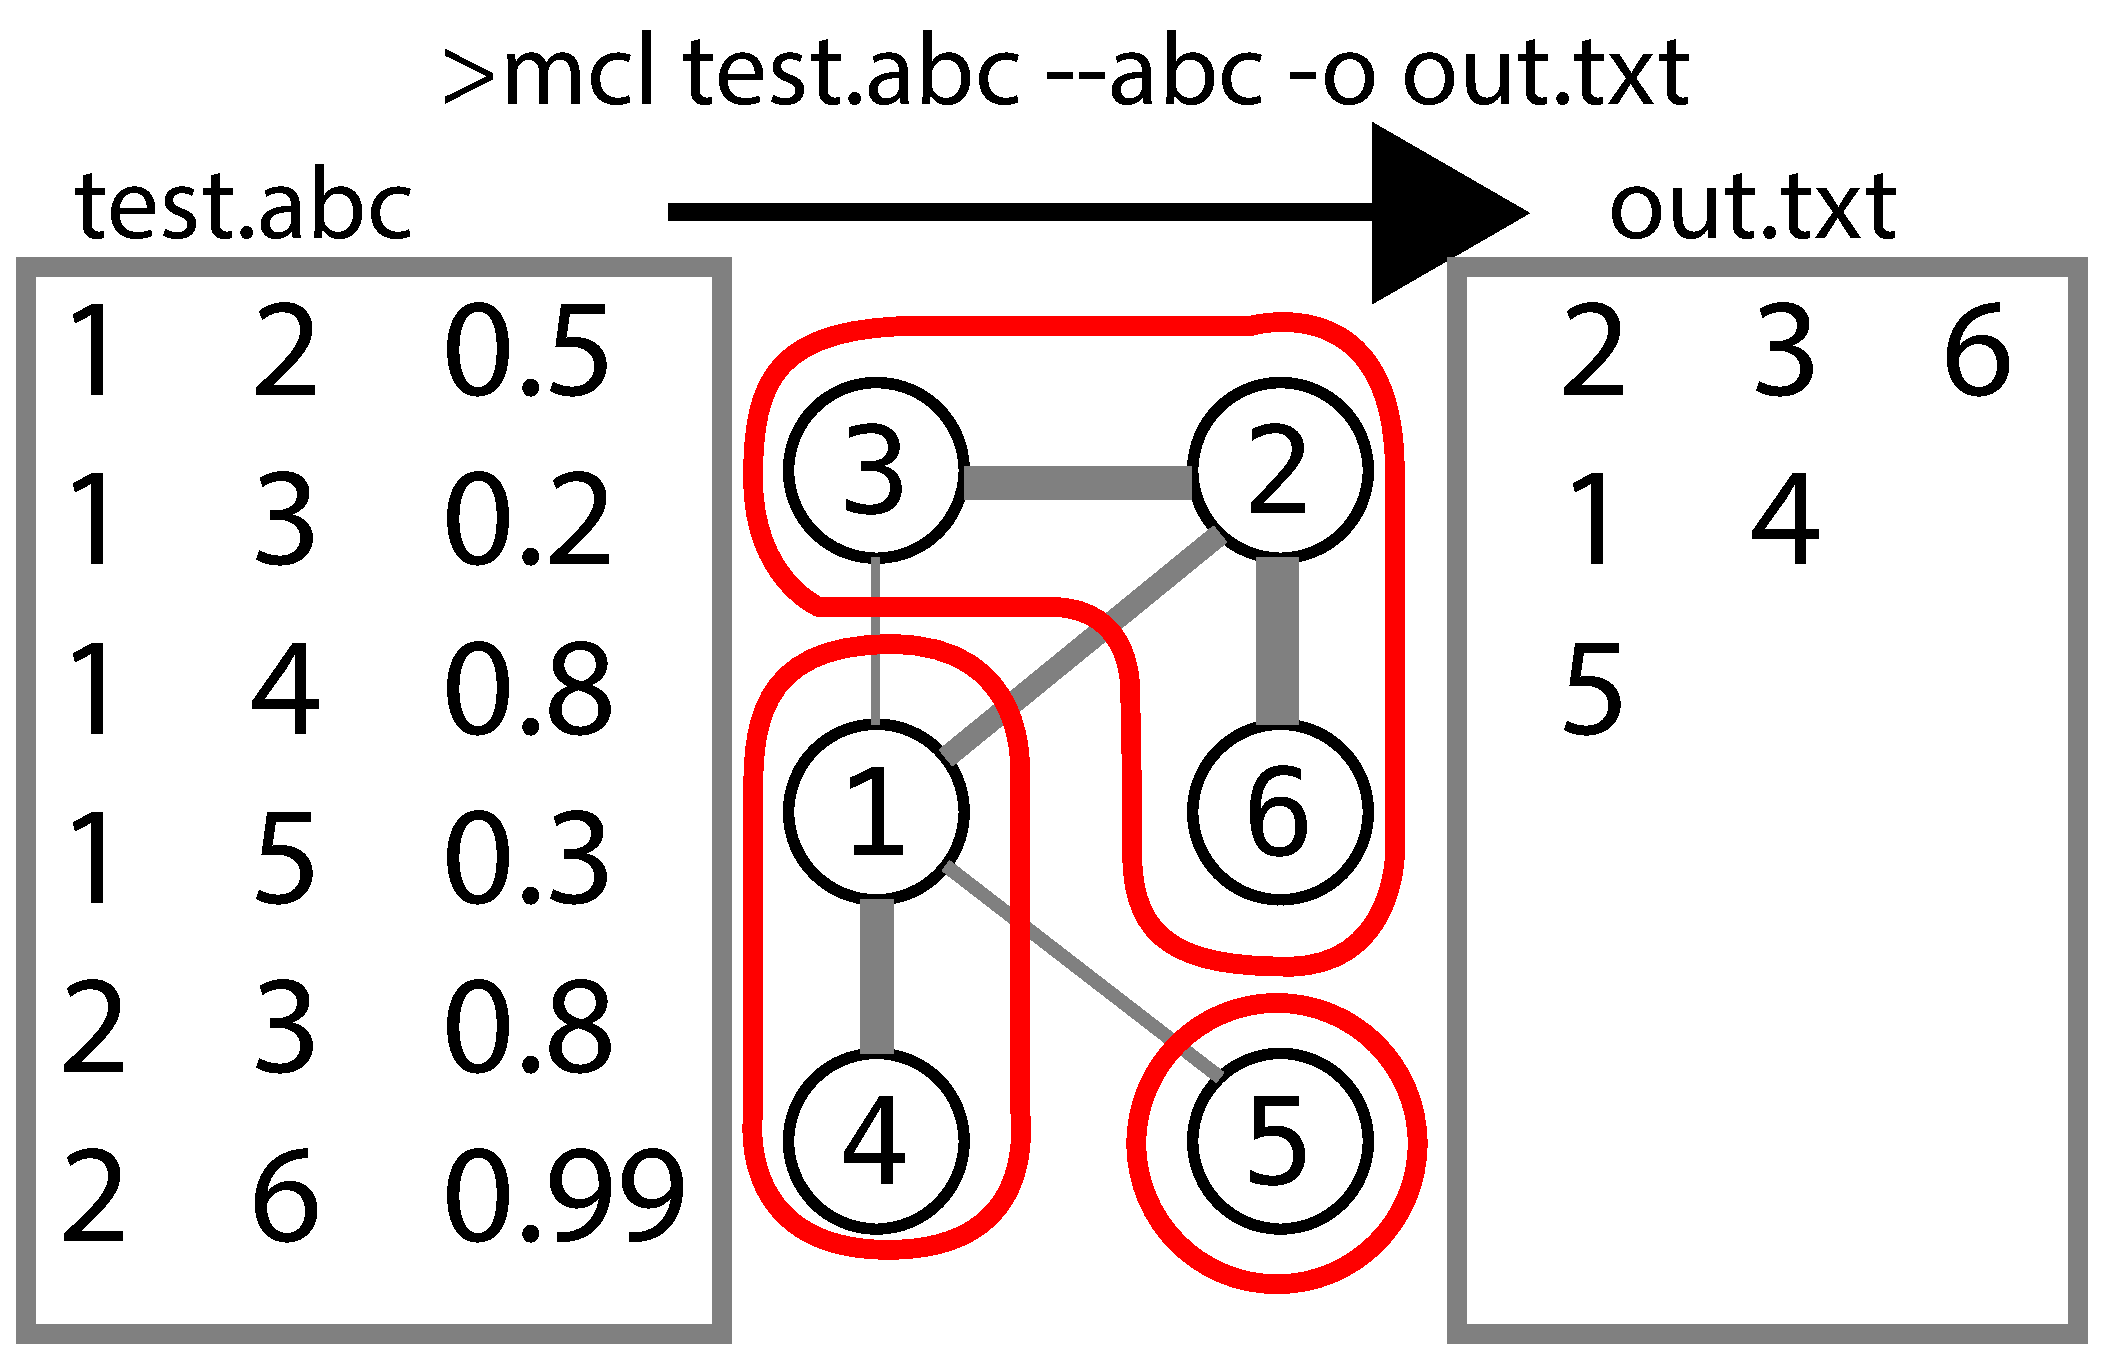
\includegraphics[scale=0.24]{nontex/illustrations/mclExample.eps}
  \label{fig:minimalMatrix}
\end{figure}
\end{frame}
\note[itemize]{
    \item has2: 4694
    \item bricsOK: 1415? 30\% or less
    \item rexOK-actual: 2871 61\%
}

%------------------------------------------------

\begin{frame}[fragile]
\frametitle{Example Cluster}

\begin{table}
\begin{center}
\caption{An example cluster containing 12 regexes, with at least one regex present in 31 different projects.  In this cluster, every regex requires `:'.}
\label{table:exampleCluster}
\begin{small}
\begin{tabular}
{lcc | lcc}
\toprule \bigstrut
\textbf{Index} & \textbf{Pattern} & \textbf{NProjects} & \textbf{Index} & \textbf{Pattern} & \textbf{NProjects} \\
 \midrule \bigstrut
1 & \begin{minipage}{1.6in}\cverb!\s*([^: ]*)\s*:(.*)!\end{minipage} & 9 & 7 & \begin{minipage}{1.6in}\cverb![:]!\end{minipage} & 6 \\
 \midrule \bigstrut
2 & \begin{minipage}{1.6in}\cverb!:+!\end{minipage} & 8 & 8 & \begin{minipage}{1.6in}\cverb!([^:]+):(.*)!\end{minipage} & 6 \\
 \midrule \bigstrut
3 & \begin{minipage}{1.6in}\cverb!(:)!\end{minipage} & 8 & 9 & \begin{minipage}{1.6in}\cverb!\s*:\s*!\end{minipage} & 4 \\
 \midrule \bigstrut
4 & \begin{minipage}{1.6in}\cverb!(:+)!\end{minipage} & 8 & 10 & \begin{minipage}{1.6in}\cverb!\:!\end{minipage} & 2 \\
 \midrule \bigstrut
5 & \begin{minipage}{1.6in}\cverb!(:)(:*)!\end{minipage} & 8 & 11 & \begin{minipage}{1.6in}\cverb!^([^:]*):[^:]*$!\end{minipage} & 2 \\
 \midrule \bigstrut
6 & \begin{minipage}{1.6in}\cverb!^([^:]*): *(.*)!\end{minipage} & 8 & 12 & \begin{minipage}{1.6in}\cverb!^[^:]*:([^:]*)$!\end{minipage} & 2 \\
\bottomrule
\end{tabular}
\vspace{-6pt}
\end{small}
\end{center}
\vspace{-12pt}
\end{table}

\end{frame}
\note[itemize]{
    \item has2: 4694
    \item bricsOK: 1415? 30\% or less
    \item rexOK-actual: 2871 61\%
}

%------------------------------------------------


\begin{frame}
\frametitle{Six Categories Of Clusters}
\begin{table}
\begin{center}
\begin{small}
\caption{Cluster categories and sizes, ordered by number of projects containing at least one pattern in the category. \label{tab:clustercats}}
\begin{tabular}{lcccc}
\toprule
\textbf{Category} & \textbf{Clusters} & \textbf{Patterns} & \textbf{Projects} & \textbf{\% Projects} \\  \midrule \bigstrut
Multi Matches & 21 & 237 & 295 & 40\% \\
\midrule \bigstrut
Specific Char & 17 & 103 & 184 & 25\% \\
\midrule \bigstrut
Anchored Patterns & 20 & 85 & 141 & 19\% \\
\midrule \bigstrut
Two or More Chars & 16 & 40 & 120 & 16\% \\
\midrule \bigstrut
Content of Parens & 10 & 46 & 111 & 15\% \\
\midrule \bigstrut
Code Search & 15 & 27 & 92 & 13\% \\
\bottomrule
\end{tabular}
\vspace{-12pt}
\end{small}
\end{center}
\end{table}




\end{frame}
\note[itemize]{
    \item partially successful
    \item did identify some use cases
    \item technique ignores 39\%
    \item technique fails to cluster similar intent, similar syntax, similar rules, labels, etc.
}

%------------------------------------------------
